\section{Project Journal}
Wordpress, an open source blogging tool, will be used to keep the project journal. A blog was chosen because it is accessible online and it provides an easy to use interface for creating multiple entries. An entry will be created for each work session as well as any important news, major ideas, part selection, design choices and implementation changes.  One advantage of this approach is that the course instructor or assistant can access the project's journal at any time to get a status update on the development and progress of this project.  The blog can be accessed at~\url{http://tinyurl.com/WaveSphere} with the password "Interfacing".

\begin{figure}[H]
	\centering
	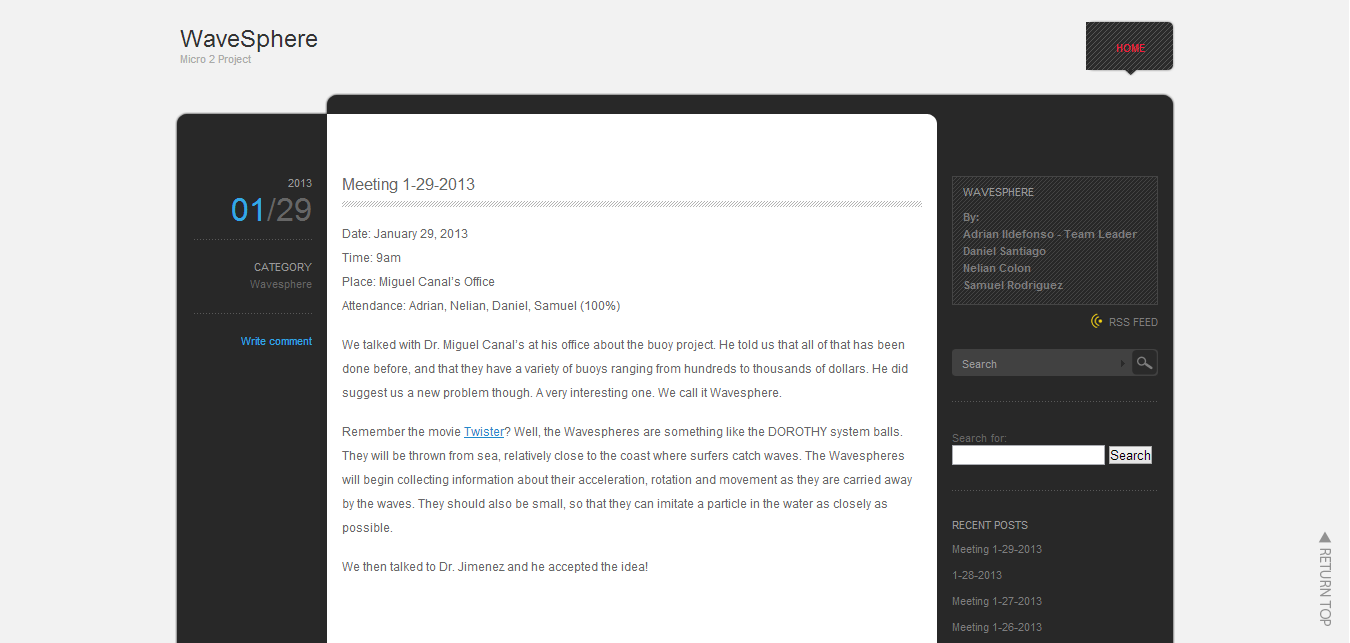
\includegraphics[scale=0.4]{img/projectJournalScreen.PNG}
	\caption{Wordpress blog \label{fig:projectJournalScreen}}
\end{figure}

